\documentclass[twocolumn]{article}



\usepackage{customization/core}



\title{Example for latex-tools}
\author{Author}

\begin{document}

\maketitle



\begin{abstract}
Dummy abstract.
\end{abstract}
 


\section{Dummy Section 1}
\label{sec:dummy1}

This is a dummy sentence~\cite{Authors14}. This is a dummy sentence~\cite{Authors14b}.
 \section{Main Text}
\label{sec:main}

\begin{figure}[t]
\centering
\begin{subfigure}[b]{0.32\linewidth}
    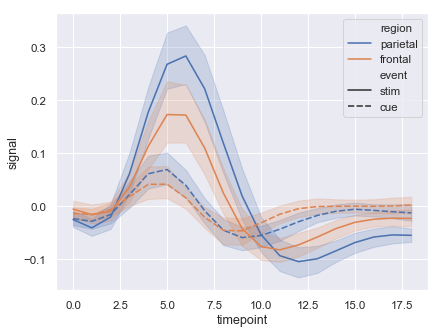
\includegraphics[width=\textwidth]{images/errorband_lineplots.png}
    \subcaption{Subfigure 1.}
    \label{fig:subcaption-subfigure1}
\end{subfigure}
\begin{subfigure}[b]{0.32\linewidth}
    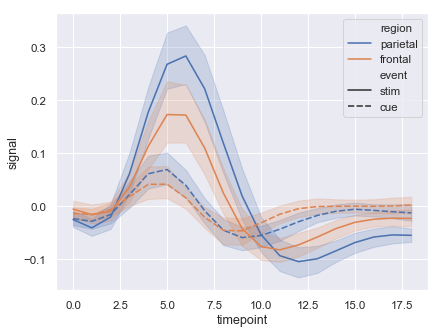
\includegraphics[width=\textwidth]{images/errorband_lineplots.png}
    \subcaption{Subfigure 2.}
    \label{fig:subcaption-subfigure2}
\end{subfigure}
\begin{subfigure}[b]{0.32\linewidth}
    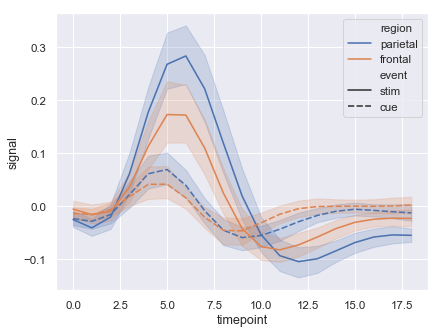
\includegraphics[width=\textwidth]{images/errorband_lineplots.png}
    \subcaption{Subfigure 3.}
    \label{fig:subcaption-subfigure3}
\end{subfigure}
\caption{Some sub-figures using \texttt{subcaption}.}
\label{fig:subcaption-subfigures}
\end{figure}
 
\begin{table}[t]
\centering
\begin{subtable}[b]{0.32\linewidth}
    \centering
    \begin{tabular}{lcr}
        \hline
        1 & 2 & 3 \\
        \hline
        4 & 5 & 6 \\
        7 & 8 & 9 \\
        \hline
    \end{tabular}
    \subcaption{Subtable 1.}
    \label{tab:subcaption-subtable1}
\end{subtable}
\begin{subtable}[b]{0.32\linewidth}
    \centering
    \begin{tabular}{lcr}
        \hline
        1 & 2 & 3 \\
        \hline
        4 & 5 & 6 \\
        7 & 8 & 9 \\
        \hline
    \end{tabular}
    \subcaption{Subtable 2.}
    \label{tab:subcaption-subtable2}
\end{subtable}
\begin{subtable}[b]{0.32\linewidth}
    \centering
    \begin{tabular}{lcr}
        \hline
        1 & 2 & 3 \\
        \hline
        4 & 5 & 6 \\
        7 & 8 & 9 \\
        \hline
    \end{tabular}
    \subcaption{Subtable 3.}
    \label{tab:subcaption-subtable3}
\end{subtable}
\caption{Some sub-tables using \texttt{subcaption}.}
\label{tab:subcaption-subtables}
\end{table}
 
Please see Fig.~\ref{fig:subcaption-subfigure1} and Table~\ref{tab:subcaption-subtable1}.
 \section{Dummy Section 2}
\label{sec:dummy2}

This is a dummy sentence~\cite{Alpher02}. This is a dummy sentence~\cite{Alpher03}. This is a dummy sentence~\cite{Alpher04}. A dummy Text\footnote{A dummy footnote.}.
  


\bibliographystyle{plain}
\bibliography{references}

\end{document}
